\documentclass[11pt,a4paper]{article}
\usepackage[margin=2.5cm]{geometry}
\usepackage{graphicx}
\usepackage{float}

\title{Report 3: Hello, CUDA!}
\author{Le Nguyen Minh Quang -- 2540093}
\date{\today}

\begin{document}
\maketitle

\section{Goal}
In this labwork I convert a color image to a gray image in two ways:
first on the CPU with a normal \texttt{for} loop, then on the GPU with
\texttt{numba.cuda}. After that I compare the time of both versions and
try different block sizes to see how they change the GPU time.

Like labwork 2, I ran the code on Google Colab because my laptop has no
NVIDIA GPU. The GPU is a \textbf{Tesla T4}. My test image is a photo of a
leaf, $549 \times 364$ pixels (199\,836 pixels in total).

\section{Method}
\begin{itemize}
  \item \textbf{Load the image:} I read the image with
  \texttt{plt.imread}. It has shape $(364, 549, 3)$, so I flatten it
  with \texttt{reshape(pixelCount, 3)}. Now each row is one pixel with
  its R, G and B values.
  \item \textbf{Gray value:} for each pixel I take the average of the
  three colors, $g = (R + G + B) / 3$, and write $g$ back to all three
  channels.
  \item \textbf{CPU version:} a simple \texttt{for} loop that goes
  through the pixels one by one.
  \item \textbf{GPU version:} each GPU thread handles one pixel. First I
  copy the image to the GPU with \texttt{cuda.to\_device}, then I launch
  the kernel, and at the end I copy the result back with
  \texttt{copy\_to\_host}. The number of blocks is
  \begin{center}
    gridSize = $\lceil$ pixelCount / blockSize $\rceil$
  \end{center}
  \item \textbf{Timing:} I used \texttt{time.time()}. I ran the kernel
  once before measuring, because the first call also compiles the
  kernel and is much slower. The GPU time includes copying the image to
  the GPU and back.
\end{itemize}

\section{Code}
\begin{verbatim}
# CPU
def grayscale_cpu(src):
    dst = np.empty_like(src)
    for i in range(pixelCount):
        g = (int(src[i, 0]) + int(src[i, 1]) + int(src[i, 2])) // 3
        dst[i, 0] = dst[i, 1] = dst[i, 2] = g
    return dst

# GPU
@cuda.jit
def grayscale_gpu(src, dst):
    tidx = cuda.threadIdx.x + cuda.blockIdx.x * cuda.blockDim.x
    if tidx < src.shape[0]:
        g = np.uint8((src[tidx, 0] + src[tidx, 1] + src[tidx, 2]) / 3)
        dst[tidx, 0] = dst[tidx, 1] = dst[tidx, 2] = g

devSrc = cuda.to_device(flatSrc)
devDst = cuda.device_array((pixelCount, 3), np.uint8)
grayscale_gpu[gridSize, blockSize](devSrc, devDst)
gpuDst = devDst.copy_to_host()
\end{verbatim}
I need the \texttt{if} in the kernel because the number of pixels is not
always a multiple of the block size. The last block can have more
threads than pixels, and those extra threads must do nothing.

\section{Results}

\subsection{CPU vs GPU (block size 64)}
\begin{center}
\begin{tabular}{|l|r|}
\hline
         & Time (ms) \\ \hline
CPU      & 256.19    \\ \hline
GPU      & 1.85      \\ \hline
\end{tabular}
\end{center}
So the GPU is about \textbf{138$\times$} faster. To check the result, I
compared the two gray images with \texttt{np.array\_equal} and they are
exactly the same. The pictures below also look the same.

\begin{figure}[H]
  \centering
  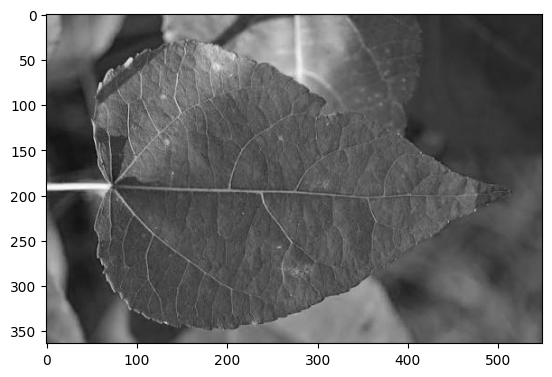
\includegraphics[width=0.48\textwidth]{gray_cpu.png}
  \hfill
  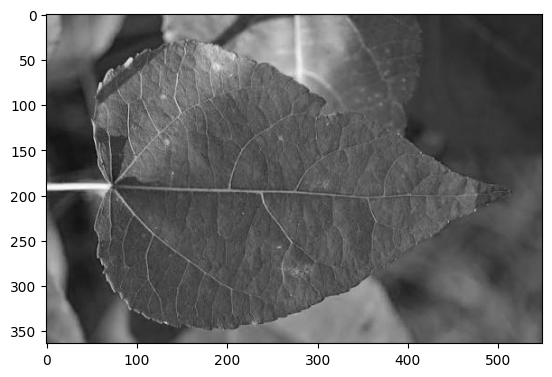
\includegraphics[width=0.48\textwidth]{gray_gpu.png}
  \caption{Gray image from the CPU (left) and from the GPU (right).}
\end{figure}

\subsection{Block size vs time}
I tried block sizes from 8 to 1024. One kernel call is very short, so
for each block size I ran the kernel 50 times and took the average.
Here I only measure the kernel, because the image is already on the GPU.

\begin{center}
\begin{tabular}{|r|r|r|}
\hline
Block size & Grid size & Kernel time (ms) \\ \hline
8    & 24980 & 0.217 \\ \hline
16   & 12490 & 0.110 \\ \hline
32   & 6245  & 0.056 \\ \hline
64   & 3123  & 0.053 \\ \hline
128  & 1562  & 0.053 \\ \hline
256  & 781   & 0.054 \\ \hline
512  & 391   & 0.054 \\ \hline
1024 & 196   & 0.057 \\ \hline
\end{tabular}
\end{center}

\begin{figure}[H]
  \centering
  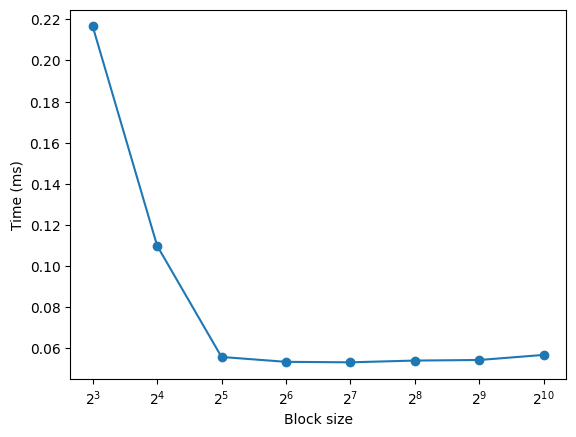
\includegraphics[width=0.7\textwidth]{blocksize_vs_time.png}
  \caption{Kernel time vs block size.}
\end{figure}

\section{Discussion}
\begin{itemize}
  \item The GPU is much faster than the CPU because it works on many
  pixels at the same time, while the CPU does them one by one.
  \item The GPU runs threads in groups of 32 (called a warp). With block
  size 8, only 8 of the 32 threads in each group do work, so it is
  about 4$\times$ slower. With 16, only half of them work, so it is
  about 2$\times$ slower.
  \item From 32 to 1024 every group is full, so the time is almost the
  same (about 0.055 ms).
\end{itemize}

\section{Conclusion}
The GPU version gives the same image as the CPU version and is about
138$\times$ faster. The block size should be at least 32 (the warp
size). After that, changing the block size does not change the time
much.

\end{document}
